\paragraph{Kinetic energy}

From second law $\vec{F}=m\frac{d\vec{v}}{dt}$.

Mathematical connection $d\vec{r} = \frac{d\vec{r}}{dt}dt = \vec{v}dt$

$$W_{A\to B} = \int_{A}^{B}\vec{F}\cdot{d\vec{r}} = \underbrace{m \int_{A}^{B} \frac{d\vec{v}}{dt} }_{\vec{F}}\cdot \underbrace{\vec{v} dt}_{d\vec{r}} = m\int_{A}^{B} \frac{1}{2}\left( \frac{dv^2}{dt} \right) dt = m \int_{A}^{B} \frac{1}{2} dv^2=\frac{1}{2}mv^2_B - \frac{1}{2}mv^2_A$$

Work equals to change in kinetic energy.

$$E_k = \frac{1}{2}mv^2$$

$$P = \frac{dW}{dt} = \vec{F} \cdot \frac{d\vec{r}}{dt} = \vec{F} \vec{v}$$

Since

$$W = \int \vec{F} \cdot d\vec{r} = \int \vec{F} \frac{d\vec{r}}{dt} dt = \int \vec{F} \vec{v} dt$$

\paragraph{Example}
$$\vec{F}_{cor} = -2 \vec{\omega} \times \vec{v}_R m$$

$$P_{cor} = \vec{F}_{cor} \cdot \vec{v}_R \stackrel{\vec{v}_R \perp \vec{\omega} \times \vec{v}_R}{=} 0$$

\paragraph{Falling mass in elevator}


\begin{center}
	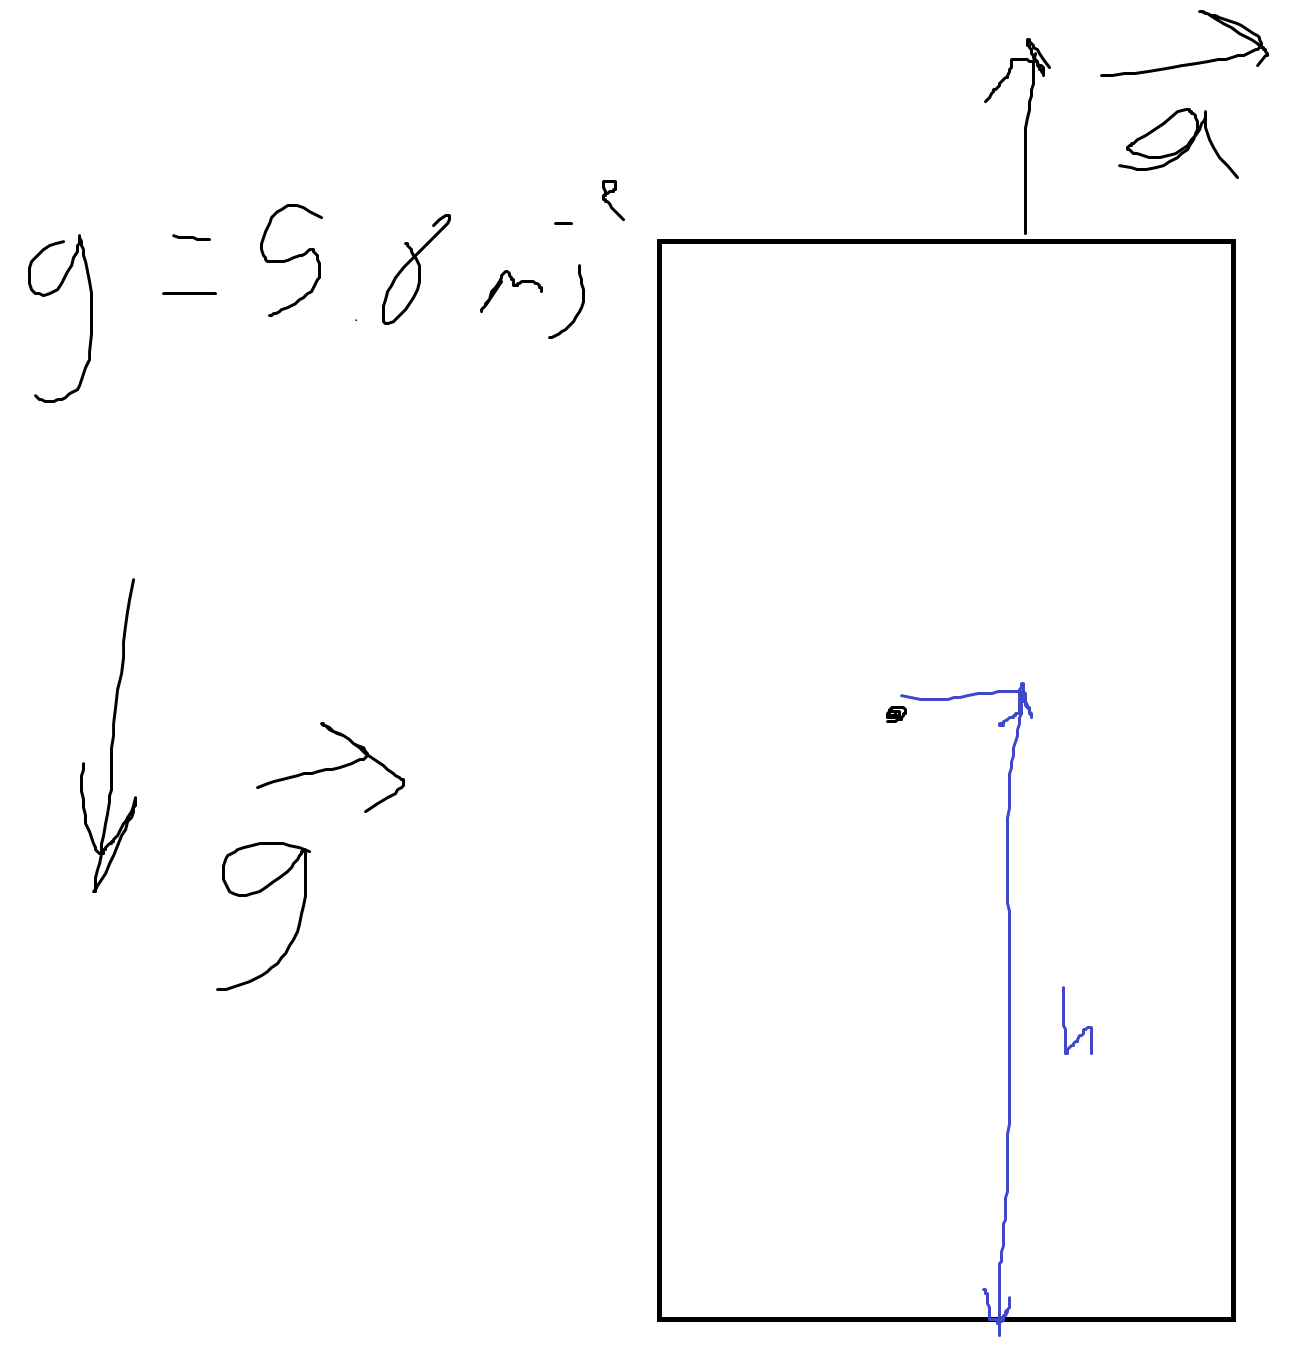
\includegraphics[width=0.2\linewidth]{./lect10/pic1.png}
\end{center}
What is final speed of falling mass?
$$g_{eff} = -(a+g)\hat{y}$$
$$v_f = \sqrt{2\left(g+a\right)h}$$

What says someone in frame of elevator?
$$U=m(g+a)h = mg_{eff}h = \underbrace{mgh}_{\parbox{2cm}{\centering \scriptsize potential energy of gravity}} + \underbrace{mga}_{\parbox{2cm}{\centering \scriptsize potential energy of acceleration due to imaginary force}}$$

\paragraph{Potential energy}
Work between two points equals to potential energy:

$$U_{\vec{r}_B}-U_{\vec{r}_A} = W_{A \to B} = \int_{A}^{B} \vec{F}_{ag} d\vec{r} $$

$$\underbrace{\vec{F}_{ag}}_{\parbox{2cm}{\centering \scriptsize Force opposite to field}} = -\vec{F}$$

$$U_{\vec{r}_B}-U_{\vec{r}_A} = \int_{A}^{B} \left(-\vec{F}\right) d\vec{r} \stackrel{cortesian}{=} -\int_A^B \left( F_x dx + F_y dy + F_z dz \right) $$

$$\vec{F} = -\left( \frac{\delta U}{\delta x}\hat{x} + \frac{\delta U}{\delta y}\hat{y} + \frac{\delta U}{\delta z}\hat{z} \right) = - \vec{\nabla} U$$

\paragraph{Conservative force} A conservative force is a force with the property that the work done in moving a particle between two points is independent of the taken path. Potential energy can be defined only for conservative force.

Also closed path results in zero work for conservative force:

$$\oint \vec{F} d\vec{r} = 0$$

\subparagraph{Examples} gravity, electricity, centrifugal in rotating system.

\paragraph{Example} Spring


\begin{center}
	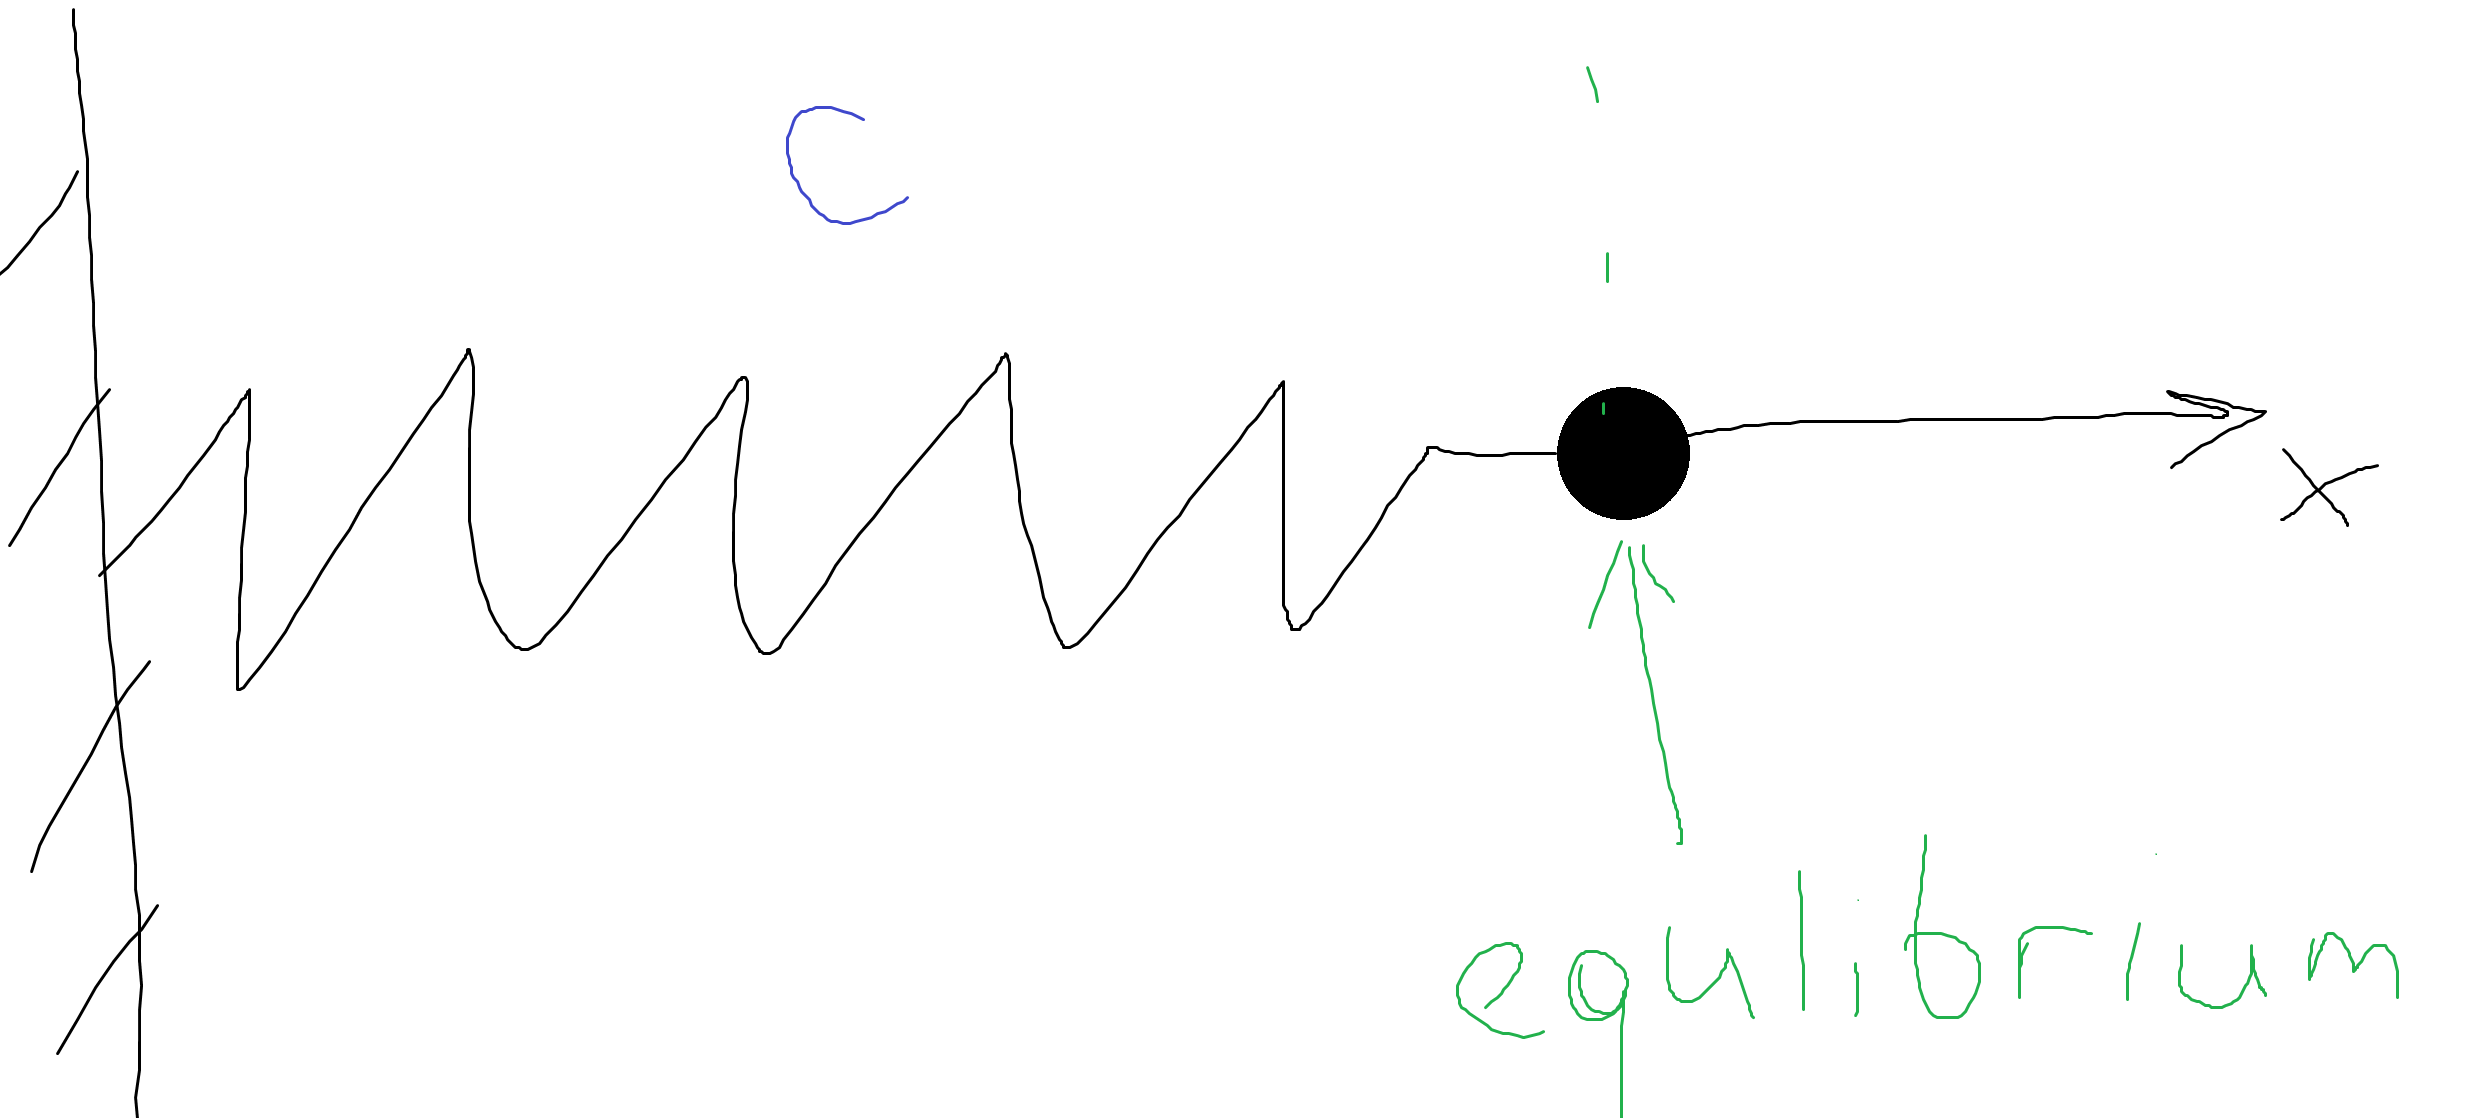
\includegraphics[width=\linewidth]{./lect10/pic2.png}
\end{center}

$$\vec{F}=-cx\hat{x}$$

where $c$ is constant of spring.

$$W_{x_1 \to x_2} = \int_{x_1}^{x_2} \underbrace{\vec{F}_{ag}}_{\parbox{2cm}{\centering \scriptsize Force opposite to spring force}} \cdot d\vec{r} = \int_{x_1}^{x_2} \left(-\vec{F}_{spring} \right) d\vec{r} $$

Since $\vec{F}_{spring} = -cx\hat{x}$ and $d\vec{r} = dx\hat{x}$

$$W_{x_1 \to x_2} = \int_{x_1}^{x_2} cx dx = \left[ cx^2 \right]_{x_1}^{x_2} = \frac{1}{2}c x_2^2 - \frac{1}{2}c x_1^2$$

Then

$$U  = \frac{1}{2}cx^2$$

and

$$\vec{F}  = -\hat{x} \frac{\delta U}{\delta x} = -cx\hat{x}$$

as expected.

\begin{center}
	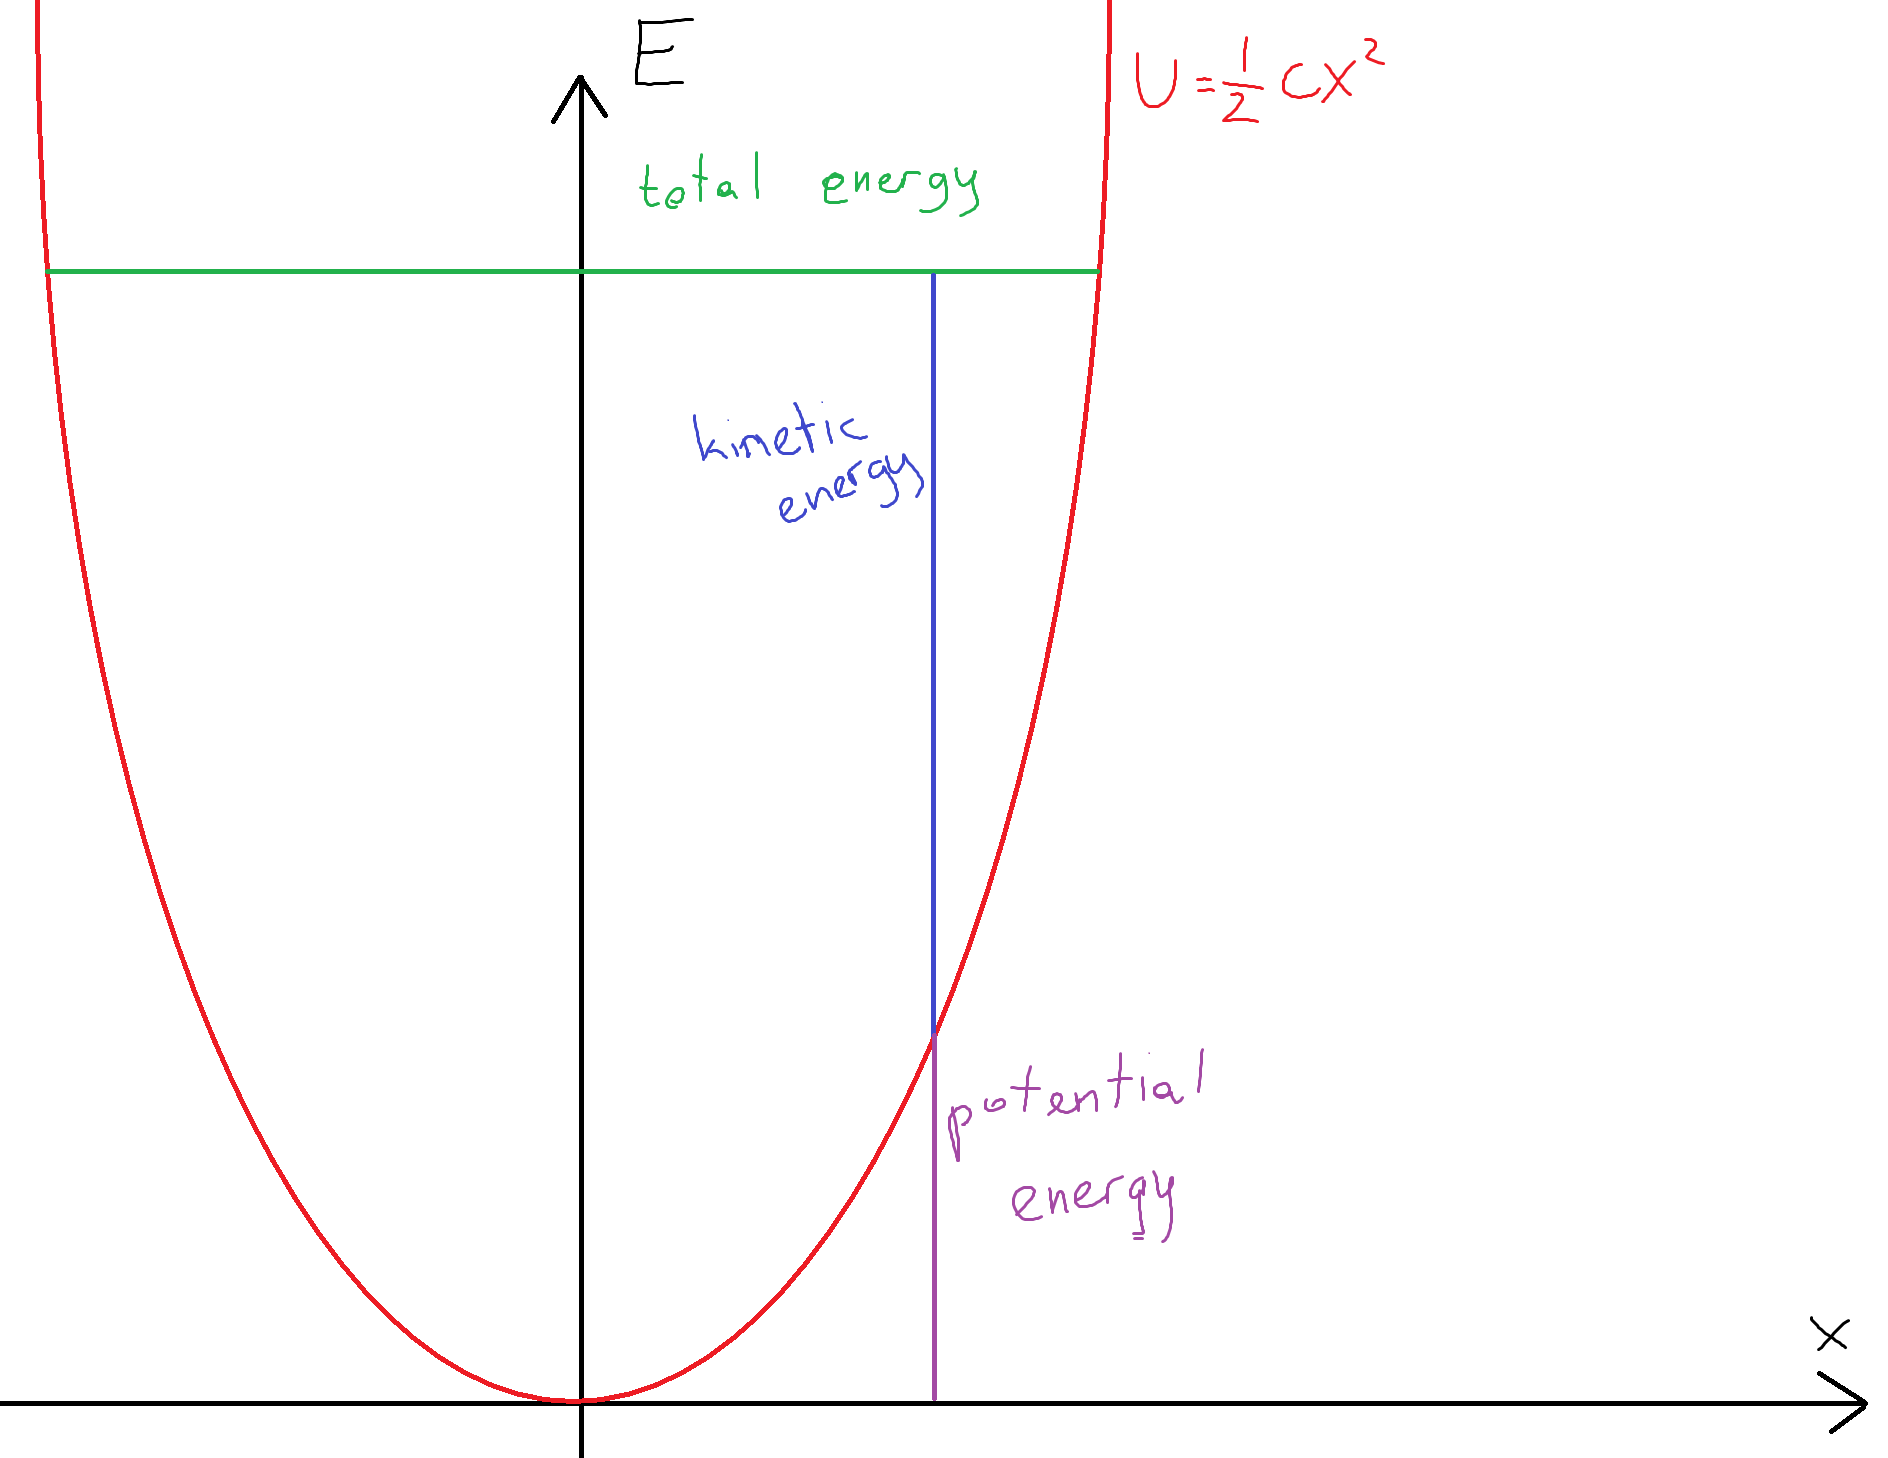
\includegraphics[width=\linewidth]{./lect10/pic3.png}
\end{center}